\section{运算后的分布}
\label{sec:rvt-output-distribution}

两枚均匀骰子的点数记为$X_1,X_2$，三十六种结果等可能。点数之和$S=X_1+X_2$取$2$到$12$之间的整数，它取各个值的概率是多少？输出的规律要从输入的规律算出来，这一节先把这件事的一般做法说清楚。

\paragraph{把目标事件写回输入}
事件“$S=7$”发生，当且仅当点数对落在
\[
 \{(1,6),(2,5),(3,4),(4,3),(5,2),(6,1)\}
\]
之中。这六个结果各有概率$1/36$，于是$\mathbb{P}(S=7)=6/36$。我们没有直接研究$S$，而是把关于$S$的事件翻译成关于$(X_1,X_2)$的事件，再用已知的联合规律计算。

图~\ref{fig:rvt-dice-sum-grid}(a)把三十六个结果画成方格，同一条斜线上的格子和相同。$S=s$对应的格子数从$s=2$的$1$个增加到$s=7$的$6$个，再减到$s=12$的$1$个，于是
\[
 \mathbb{P}(S=s)=\frac{6-\lvert s-7\rvert}{36},\qquad s=2,3,\ldots,12 .
\]
十一个概率之和是$(1+2+\cdots+6+5+\cdots+1)/36=1$。

\begin{BookInlineFigure}
  \centering
  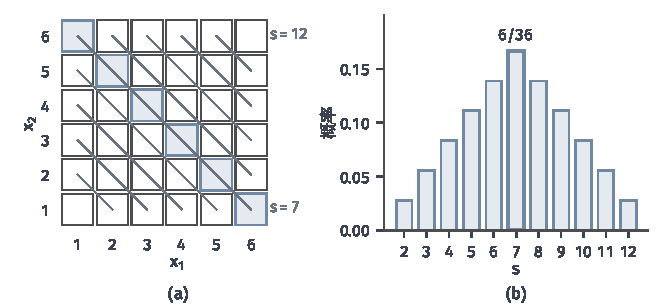
\includegraphics[width=112mm]{figures/07-probability/01-elementary-probability/matplotlib/rvt-dice-sum-grid/figure.pdf}
  \caption{两枚骰子之和。(a)三十六个等可能结果，灰线连接和相同的格子，蓝色格子是事件$S=7$的原像。(b)$S$的概率质量，第$s$根柱的高度等于(a)中第$s$条斜线上的格子数除以$36$。}
  \label{fig:rvt-dice-sum-grid}
\end{BookInlineFigure}

\paragraph{原像规则}
设$X$是一个随机变量或随机向量，$g$是定义在其取值范围上的确定函数，$Y=g(X)$。对输出的一个取值集合$B$，输入的\term{原像}（preimage）是
\[
 g^{-1}(B)=\{x:\ g(x)\in B\} .
\]
这里$g^{-1}(B)$只是一个集合的记号，$g$不必可逆。事件“$Y\in B$”与“$X\in g^{-1}(B)$”由同样的试验结果组成，所以它们的概率相等：
\begin{equation}
 \mathbb{P}(Y\in B)=\mathbb{P}\bigl(X\in g^{-1}(B)\bigr) .
 \label{eq:rvt-preimage-rule}
\end{equation}
多个输入的情形完全一样，只是把$X$换成随机向量$(X_1,\ldots,X_n)$，右端用联合分布计算。

式~\eqref{eq:rvt-preimage-rule}在两种模型下分别落成求和与积分。$X$离散时，取$B=\{y\}$，原像是所有被送到$y$的输入，于是
\begin{equation}
 p_Y(y)=\sum_{x:\ g(x)=y}p_X(x) .
 \label{eq:rvt-discrete-pushforward}
\end{equation}
$X$有密度$f_X$时，取$B=(-\infty,y]$，得到输出的分布函数
\begin{equation}
 F_Y(y)=\int_{\{x:\ g(x)\leq y\}}f_X(x)\,\mathrm{d}x .
 \label{eq:rvt-cdf-method}
\end{equation}
这里的集合$B$取区间、区域等前几章能计算概率的集合；哪些集合都能这样处理，在第~\ref{chap:probability-spaces}章统一说明。

\paragraph{搬运质量的图景}
把概率看成总量为$1$的质量，式~\eqref{eq:rvt-discrete-pushforward}说的是：每个输入格子把自己的质量搬到$g$指定的输出位置，落在同一位置的质量相加。图~\ref{fig:rvt-dice-sum-grid}中，一条斜线上的六个格子把质量都搬到$7$，所以$7$处堆得最高。

这个图景在连续情形要补一句。密度是单位长度上的质量，质量被搬走时如果所占的长度被拉长或压短，单位长度上的质量就要相应变小或变大。式~\eqref{eq:rvt-cdf-method}只算总质量，不受这一点影响；从它求密度时，伸缩就会出现在公式里，这是下一节的主题。

\paragraph{分布与函数期望}
第~\ref{chap:random-variable-moments}章计算$\mathbb{E}[g(X)]$时直接对$X$的分布加权，不先求$g(X)$的分布。骰子的例子里
\[
 \mathbb{E}[S]=\sum_{x_1=1}^{6}\sum_{x_2=1}^{6}\frac{x_1+x_2}{36}=7 .
\]
两种算法给出同一个结果。按式~\eqref{eq:rvt-discrete-pushforward}，把输入按$g(x)$的值分组，组内的$g(x)$都等于同一个$y$：
\[
 \sum_{x}g(x)\,p_X(x)=\sum_{y}\ y\sum_{x:\ g(x)=y}p_X(x)=\sum_{y}y\,p_Y(y) .
\]
分组只是改变了加法的次序；无穷多项时这一步要求级数绝对收敛，这正是期望存在的条件。

两件事回答的问题不同。一个期望只是分布的一个数值，知道$\mathbb{E}[S]=7$不能推出$\mathbb{P}(S\geq10)$。反过来，输出分布确定了$Y$的每一个函数的期望，例如
\[
 \mathbb{P}(S\geq10)=\mathbb{E}\bigl[\mathbf{1}_{\{S\geq10\}}\bigr]=\frac{3+2+1}{36}=\frac16 .
\]
要回答关于$Y$的所有概率问题，就需要求出$Y$的分布；只要一两个平均值时，直接按第~\ref{chap:random-variable-moments}章计算更省事。

\paragraph{独立性的保持}
把四枚骰子分成两组，前两枚的点数和$S=X_1+X_2$与后两枚的较大值$M=\max(X_3,X_4)$是否独立？直觉上是：两组骰子互不影响，各自算出的量也互不影响。下面的定理说明这个直觉在什么条件下成立。

称随机向量$\bm{U}=(X_1,\ldots,X_k)$与$\bm{W}=(X_{k+1},\ldots,X_n)$相互独立，是指它们的联合概率质量（或联合密度）等于两组各自联合质量（或密度）的乘积。$X_1,\ldots,X_n$相互独立时，第~\ref{chap:random-vectors}章的乘积分解按组归并，就得到这一点。

\begin{theorem}[分组变换保持独立]
\label{thm:rvt-group-independence}
设$\bm{U}$与$\bm{W}$相互独立，$g$、$h$是确定的函数。则对能计算概率的取值集合$A$、$B$，
\begin{equation}
 \mathbb{P}\bigl(g(\bm{U})\in A,\ h(\bm{W})\in B\bigr)=\mathbb{P}\bigl(g(\bm{U})\in A\bigr)\,\mathbb{P}\bigl(h(\bm{W})\in B\bigr) .
 \label{eq:rvt-group-independence}
\end{equation}
即$g(\bm{U})$与$h(\bm{W})$相互独立。
\end{theorem}

\begin{proof}
记$A'=g^{-1}(A)$，$B'=h^{-1}(B)$。由原像规则，左端的事件就是$\bm{U}\in A'$且$\bm{W}\in B'$。

离散情形，联合质量写成$p_{\bm{U}}(\bm{u})\,p_{\bm{W}}(\bm{w})$，对$\bm{u}\in A'$、$\bm{w}\in B'$求和。二重和中的每一项是两个因子的乘积，第一个只依赖$\bm{u}$，第二个只依赖$\bm{w}$，所以
\[
 \sum_{\bm{u}\in A'}\sum_{\bm{w}\in B'}p_{\bm{U}}(\bm{u})\,p_{\bm{W}}(\bm{w})=\Bigl(\sum_{\bm{u}\in A'}p_{\bm{U}}(\bm{u})\Bigr)\Bigl(\sum_{\bm{w}\in B'}p_{\bm{W}}(\bm{w})\Bigr) .
\]
右端两个因子分别是$\mathbb{P}(\bm{U}\in A')$与$\mathbb{P}(\bm{W}\in B')$，再用一次原像规则，就是式~\eqref{eq:rvt-group-independence}的右端。

有密度时把求和换成积分。积分区域是乘积集合$A'\times B'$，被积函数是$f_{\bm{U}}(\bm{u})f_{\bm{W}}(\bm{w})$，按累次积分先对$\bm{w}$、后对$\bm{u}$积分，内层积分与$\bm{u}$无关，可以提到外面，得到同样的乘积。
\end{proof}

证明只用到一件事：两组输入的联合规律可以分解，而$g$只读第一组、$h$只读第二组，于是两个原像分别落在乘积的两个因子里。所以$S$与$M$独立。

条件中的“分组”不能省。$S=X_1+X_2$与$D=X_1-X_2$都只由前两枚骰子算出，但它们读的是同一组输入。$S=2$迫使两枚骰子都是$1$，于是$D=0$；所以
\[
 \mathbb{P}(S=2,\ D=1)=0,\qquad \mathbb{P}(S=2)\,\mathbb{P}(D=1)=\frac{1}{36}\cdot\frac{5}{36}>0 ,
\]
$S$与$D$不独立。

\paragraph{边缘分布的不足}
没有独立结构时，只知道每个输入各自的分布，输出的分布通常还不确定。最小的例子是两个只取$0,1$的变量$X,Y$，各自都满足$\mathbb{P}(X=1)=\mathbb{P}(Y=1)=1/2$。下面三种联合规律都与这两个边缘相容：
\begin{itemize}
 \item 独立：四个格子各有$1/4$，和$X+Y$取$0,1,2$的概率是$1/4,1/2,1/4$；
 \item 完全一致，$Y=X$：质量只在$(0,0)$与$(1,1)$，和取$0,2$各$1/2$；
 \item 完全相反，$Y=1-X$：质量只在$(0,1)$与$(1,0)$，和恒等于$1$。
\end{itemize}

图~\ref{fig:rvt-same-marginals}把三张概率表和对应的和画在一起。三张表的行和与列和都是$(1/2,1/2)$，和的期望都是$1$，可是和的分布从“三点”变成“两点”，再变成一个确定的数。

\begin{BookInlineFigure}
  \centering
  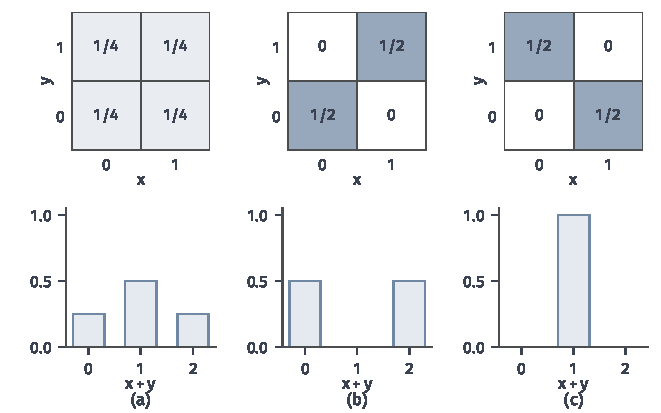
\includegraphics[width=112mm]{figures/07-probability/01-elementary-probability/matplotlib/rvt-same-marginals/figure.pdf}
  \caption{相同边缘、不同联合规律下的和。上排是$(X,Y)$的三张概率表，格中数字与蓝色深浅表示概率，三张表的行和与列和都是$1/2$。下排是对应的$X+Y$的概率质量：(a)独立，(b)$Y=X$，(c)$Y=1-X$。}
  \label{fig:rvt-same-marginals}
\end{BookInlineFigure}

原因在原像。事件$X+Y=1$的原像是两个对角格子$\{(0,1),(1,0)\}$，边缘分布只规定行和与列和，对角格子上的质量可以在$0$到$1/2$之间任意选。所以计算输出分布时要先确认用的是联合规律；只有在独立时，联合规律才能由边缘相乘得到。后面讲和、乘积、比值时都会把一般公式与独立情形分开写。
